\subsubsection{UC7 - Login automatico}
\begin{figure}[H]
	\centering
	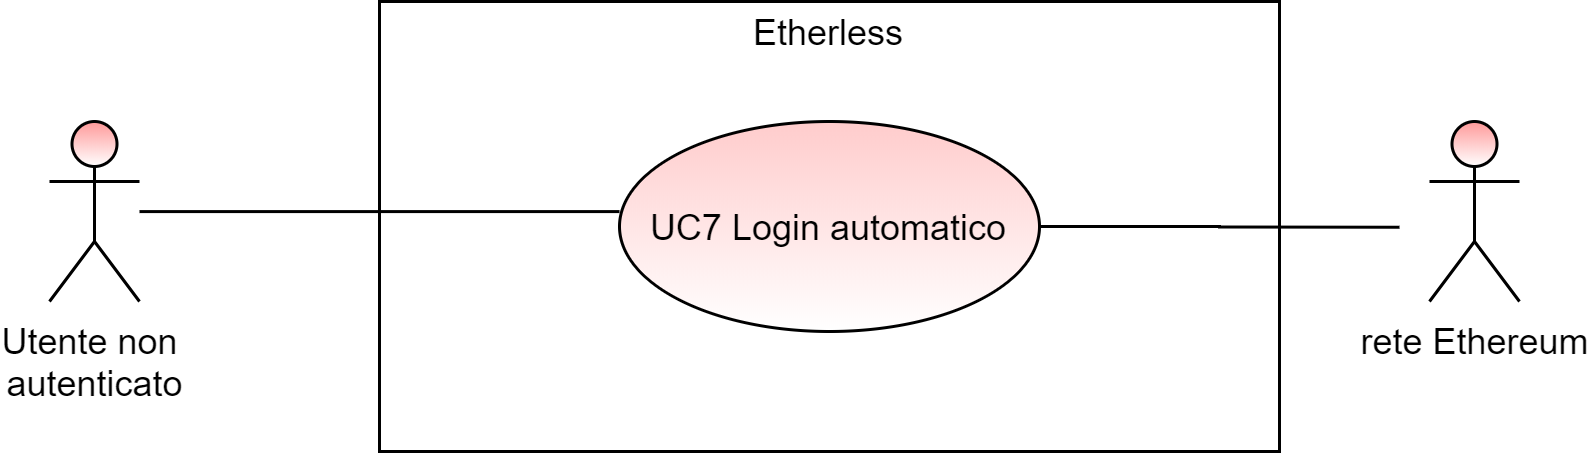
\includegraphics[scale=\ucs]{./res/img/UC7G.png}
	\caption {UC7 - Login automatico: schema generale}
\end{figure}
\begin{itemize}
	\item \textbf{Attori primari:} \una{};
	\item \textbf{Attori secondari:} \re{};
	\item \textbf{Descrizione:} in maniera automatica il sistema si occupa dell’autenticazione dell’utente;
	\item \textbf{Scenario principale:} l’utente avvia l'applicativo tramite il comando \init{} e viene autenticato in maniera automatica; 
	\item \textbf{Precondizione:} l’utente ha eseguito il login manuale almeno una volta, indicando esplicitamente la volontà di essere ricordato [\textbf{UC6}];
	\item \textbf{Postcondizione:} l’utente si è autenticato con successo.
\end{itemize}